\section{Vehicle Modeling with Chronos}
\label{vehicle_modeling_chronos}

In this section we will develop and simulate a vehicle model using the open source physics engine \lstinline{chronos}.

\begin{lstlisting}
http://projectchrono.org/
\end{lstlisting}
 
Specifically, we will simulate a vehicle that moves in straight line.  Figure \ref{straight_line_motion} shows a snapshot of the simulation

\begin{figure}[!htb]
\begin{center}
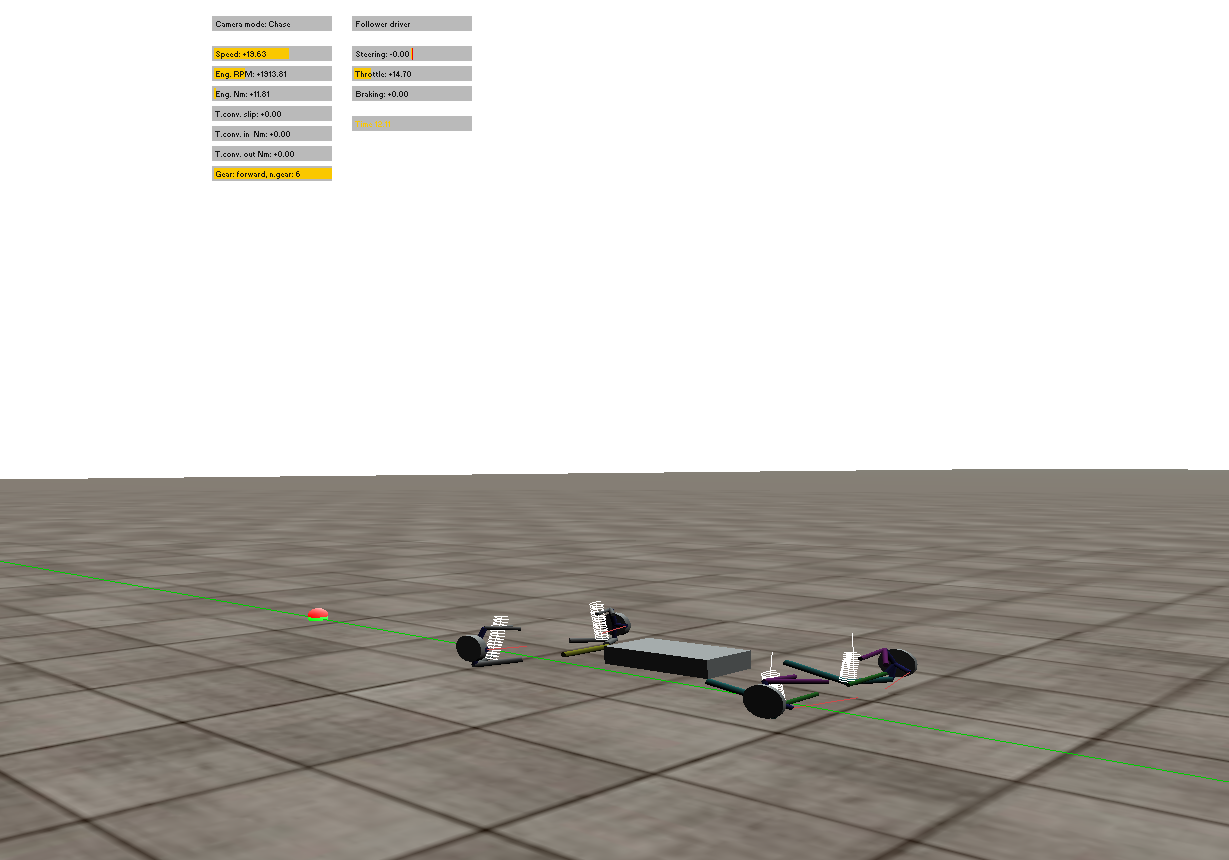
\includegraphics[scale=0.290]{img/straight_line_motion.png}
\end{center}
\caption{Straight line vehicle motion.}
\label{straight_line_motion}
\end{figure}

The following link can be used to consult for further information 
\begin{lstlisting}
http://api.projectchrono.org/tutorial_install_project.html
\end{lstlisting}

The reference manual can be found at
\begin{lstlisting}
http://api.projectchrono.org/manual_root.html
\end{lstlisting}
\subsection{The \lstinline{Chrono::Vehicle} library}

The \lstinline{Chrono::Vehicle} is a C++ middleware library for the modeling, simulation, and visualization of wheeled and tracked ground vehicles.
It consists of two core modules:

\begin{itemize}
\item The \lstinline{ChronoEngine_vehicle}

	\begin{itemize}
		\item Defines the system and subsystem base classes
		\item Provides concrete, derived classes for instantiating templates from JSON specification files
		\item Provides miscellaneous utility classes and free functions for file I/O, Irrlicht vehicle visualization, steering and speed controllers, vehicle and subsystem test rigs, etc.
	\end{itemize}

\item The \lstinline{ChronoModels_vehicle}
	\begin{itemize}
		\item Provides concrete classes for instantiating templates to model specific vehicle models
	\end{itemize}
\end{itemize}

The following dependencies should be satisfied in order to use the library.

\begin{itemize}
\item The \lstinline{Chrono::Engine } required
\item The \lstinline{Chrono::Irrlicht} and the \lstinline{Irrlicht} library,  \lstinline{Chrono::OpenGL} and its dependencies. Both are optional
\item The \lstinline{Chrono::FEA} and \lstinline{Chrono::MKL} (optional)
\end{itemize}

The \lstinline{Chrono::Engine } supports the notion of a system. In our case, the following components are considered a system

\begin{itemize}
\item Powertrain
\item Tire
\item Terrain
\item Driver
\item Vehicle
\end{itemize}

\lstinline{Chrono::Vehicle} encapsulates templates for systems and subsystems in polymorphic C++ classes:

\begin{itemize}
\item A base abstract class for the system/subsystem type (e.g. \lstinline{Chrono::ChSuspension})
\item A derived, still abstract class for the system/subsystem template (e.g.  \lstinline{Chrono::ChDoubleWishbone})
\item Concrete class that particularize a given system/subsystem template (e.g. \lstinline{Chrono::HMMWV_DoubleWishboneFront})
\end{itemize}

\subsection{The \lstinline{chrono::vehicle::ChVehicle} class}

Vehicles in \lstinline{Chrono} inherit from the base class \lstinline{chrono::vehicle::ChVehicle}. 
This class provides the interface between the vehicle system and other systems (tires, driver, etc.)

The reference frame for a vehicle follows the ISO standard. 
Namely, $Z$-axis up, $X$-axis pointing forward, and $Y$-axis towards the left of the vehicle. The following figure illustrates
the asseumed reference frames.


\begin{figure}[!htb]
\begin{center}
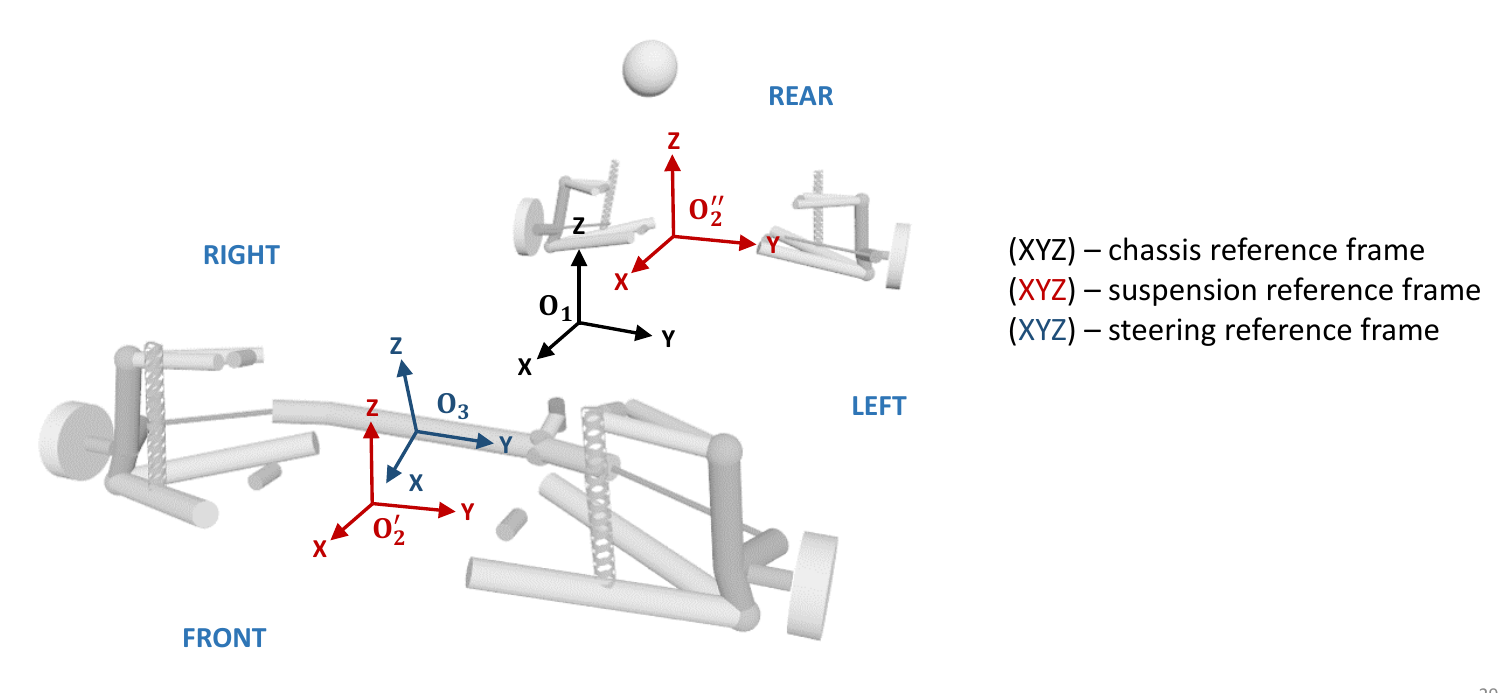
\includegraphics[scale=0.290]{img/vehicle_iso_ref_frame.jpeg}
\end{center}
\caption{Vehicle ISO reference frames.}
\label{vehicle_iso_ref_frame}
\end{figure}

A \lstinline{chrono::vehicle::ChVehicle} has

\begin{itemize}
\item \lstinline{ChSystem* m_system} pointer to the Chrono system
\item \lstinline{std::shared_ptr<ChChassis> m_chassis} handle to the chassis subsystem
\item \lstinline{bool m_ownsSystem} true if system created at construction
\item \lstinline{double m_stepsize}  integration step-size for the vehicle system
\end{itemize}

Deferring to its constituent subsystems as needed, a \lstinline{chrono::vehicle::ChVehicle} provides accessors for:

\begin{itemize}
\item Underlying \lstinline{chrono::vehicle::ChSystem}
\item Handle to the vehicle chassis
\item Chassis state (reference frame and COM)
\item Angular speed of the vehicle driveshaft (connection to powertrain)
\end{itemize}

A \lstinline{chrono::vehicle::ChVehicle} intermediates communication between other systems (e.g.,
powertrain, driver, etc.) and constituent subsystems (e.g., suspensions, brakes, etc.)

\subsection{ The \lstinline{chrono::vehicle::ChChassis} class}

This is the ase class for the chassis vehicle subsystem. The class documentation can be found at 

\begin{lstlisting}
http://api.projectchrono.org/classchrono_1_1vehicle_1_1_ch_chassis.html
\end{lstlisting}

A chassis has the following attributes

\begin{itemize}
\item \lstinline{std::shared_ptr<ChBodyAuxRef> m_body}; a handle to the chassis body
\item \lstinline{bool m_fixed}; a flag indicating if the chassis body is fixed to the ground
\end{itemize}

It provides access to the following properties

\begin{itemize}
\item Chassis mass and inertia properties
\item Chassis state reference frame and COM
\item Vehicle speed reference frame and COM
\item Driver position
\item Absolute acceleration of a point specified in local reference frame
\end{itemize}

A chassis system can be specified in a JSON file.

\subsection{ The \lstinline{chrono::vehicle::ChDriver} class}

Base class for a vehicle driver system.
A driver system must be able to report the current values of the inputs (throttle, steering, braking). 
A concrete driver class must set the member variables:

\begin{itemize}
\item \lstinline{m_throttle}
\item \lstinline{m_steering} 
\item \lstinline{m_braking}
\end{itemize}
Since these are the main quantities that a driver can interact with a vehicle, this class has to be adapted
when we want to incorporate autonomy. 


\subsection{Setup simulation}

\subsubsection{Setup the vehicel \lstinline{chrono::vehicle::sedan::Sedan}}

Now that we went over the basics of the \lstinline{Chrono::Vehicle} library let's try to set up a basic simulation; namely a vehicle that moves in straight line.
Concretely, we will use an instance of the \lstinline{chrono::vehicle::sedan::Sedan} class. 



The following code initializes the vehicle instance for the simulation

\begin{lstlisting}
// Create the vehicle, set parameters, and initialize
    Sedan vehicle;
    vehicle.SetContactMethod(contact_method);
    vehicle.SetChassisFixed(false);
    vehicle.SetInitPosition(ChCoordsys<>(initLoc, initRot));
    
    vehicle.SetTireType(tire_model);
    vehicle.SetTireStepSize(tire_step_size);
    vehicle.SetVehicleStepSize(step_size);
    vehicle.Initialize();

    vehicle.SetChassisVisualizationType(chassis_vis_type);
    vehicle.SetSuspensionVisualizationType(suspension_vis_type);
    vehicle.SetSteeringVisualizationType(steering_vis_type);
    vehicle.SetWheelVisualizationType(wheel_vis_type);
    vehicle.SetTireVisualizationType(tire_vis_type);
\end{lstlisting}


\subsubsection{Create the application}

\begin{lstlisting}
// Create the vehicle Irrlicht application
ChVehicleIrrApp app(&vehicle.GetVehicle(), &vehicle.GetPowertrain(), 
		    L"Steering XT Controller Demo", 
        irr::core::dimension2d<irr::u32>(800, 640));

app.SetHUDLocation(500, 20);
app.SetSkyBox();
app.AddTypicalLogo();

irr::core::vector3df v1(-150.f, -150.f, 200.f);
irr::core::vector3df v2(-150.f, 150.f, 200.f);
irr::core::vector3df v3(150.f, -150.f, 200.f);
irr::core::vector3df v4(150.0f, 150.f, 200.f); 
app.AddTypicalLights(v1, v2, 100, 100);
app.AddTypicalLights(v3, v4, 100, 100);
app.EnableGrid(false);
app.SetChaseCamera(trackPoint, 6.0, 0.5);
app.SetTimestep(step_size);
\end{lstlisting}

Our application will use an instance of the \lstinline{Chrono::ChPathFollowerDriverXT} class. This is a driver model that uses a path steering controller and a speed controller. The steering controller adjusts the steering input to follow the prescribed path. 
The output from the speed controller is used to adjust throttle and braking inputs in order to maintain the prescribed constant vehicle speed.


\subsubsection{Advance the vehicle}

Each system base class declares a virtual function \lstinline{Advance()}
with a single parameter, the time interval between two communication points $(\Delta t)$.
A particular system may take as many intermediate steps (constant or variable step-size) 
as needed to advance the state of the system by $(\Delta t)$.  If the system has no internal dynamics, this function can be a no-op

\begin{lstlisting}
driver_follower.Advance(step);
driver_gui.Advance(step);
terrain.Advance(step);
vehicle.Advance(step);
app.Advance(step);
\end{lstlisting}


\subsubsection{Vehicle state information}

When running a simulation, we would like to be able to view various quantites that describe the state of the vehicle. Let's see how
we can obtain some of them.

\textbf{Get the vehicle position coordinates and vehicle speed}

\begin{lstlisting}
//This is the global location of the chassis reference frame origin. 
ChVector<> pos = vehicle.GetVehicle().GetVehiclePos();

//Return the speed measured at the origin of the chassis reference frame.
double speed = vehicle.GetVehicle().GetVehicleSpeed();
\end{lstlisting}












